\documentclass[../../main.tex]{subfiles}

\begin{document}

Sea la siguiente tabla un contexto formal $(G, M, I)$, donde $G$ es el conjunto de los objetos $\{ o1, o2, o3, o4, o5, o6 \}$, 
$M$ es el conjunto de los atributos $\{ a1, a2, a3, a4, a5 \}$ y $I \subseteq G \times M$ es la relación binaria entre $G$ y $M$.

\begin{table}[H]
    \begin{center}
    \begin{tabular}{|c|c|c|c|c|c|}
    \hline
    \multicolumn{1}{|l|}{} & \multicolumn{1}{l|}{a1} & \multicolumn{1}{l|}{a2} & \multicolumn{1}{l|}{a3} & \multicolumn{1}{l|}{a4} & \multicolumn{1}{l|}{a5} \\ \hline
    o1                     &                         & x                       & x                       &                         & x                       \\ \hline
    o2                     & x                       &                         & x                       & x                       &                         \\ \hline
    o3                     & x                       & x                       & x                       & x                       &                         \\ \hline
    o4                     & x                       &                         &                         & x                       &                         \\ \hline
    o5                     & x                       & x                       & x                       & x                       &                         \\ \hline
    o6                     & x                       &                         & x                       & x                       &                         \\ \hline
    \end{tabular}
    \end{center}
    \caption{Objetos / Atributos}
\end{table}

Usando los operadores de derivación podemos calcular las imágenes de conjuntos de objetos y atributos, algunos ejemplos:

\begin{itemize}
    \item $\{ o2 \}^{'} = \{ a1, a3, a4 \}$ 
    \item $\{ a3 \}^{'} = \{ a1, a2, a3, a5, a6 \}$ 
    \item $\{ o3, o5 \}^{'} = \{ a1, a2, a3, a4 \}$ 
    \item $\{ a3, a4 \}^{'} = \{ o2, o3, o5, o6 \}$ 
\end{itemize}

Los operadores de derivación pueden ser iterados, es decir, si partimos de un conjunto $A \subseteq G$, es posible obtener $A^{'}$ que es un subconjunto de $M$. Si aplicamos el segundo operador de derivación, obtenemos $(A^{'})^{'}$ o $A^{''}$, que es un conjunto de objetos. Si seguimos con el proceso de iteración, podemos obtener $A^{'''}$, $A^{''''}$ y así sucesivamente.

\begin{itemize}
    \item $\{ o3 \}^{''} = \{ a1,a2,a3,a4 \}^{'} = \{ o3, o5 \}$ 
    \item $\{ o1,o3,o5 \}^{''} = \{ a2,a3 \}^{'} = \{ o1,o3,o5 \}$  
    \item $\{ a3,a4 \}^{''} = \{ o2,o3,o5,o6 \}^{'} = \{ a1,a3,a4 \}$ 
    \item $\{ a3 \}^{''} = \{ o1,o2,o3,o5,o6 \}^{'} = \{ a3 \}$ 
\end{itemize}

Con esto se construye el siguiente retículo de conceptos:
\begin{figure}[H]
\centering
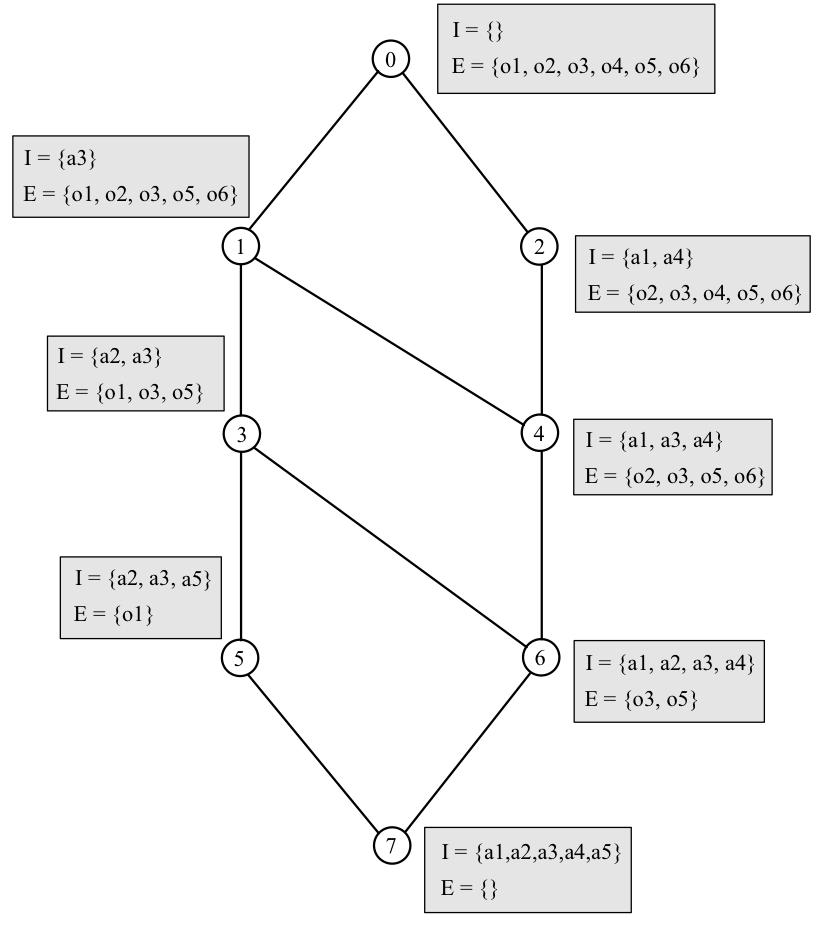
\includegraphics[width=0.75\textwidth]{images/fca/reticulo1.png}
\caption{Retículo de conceptos del Ejemplo 1}
\end{figure}

Donde $I$ es el conjunto de intenciones y $E$ es el conjunto de extensiones.

\end{document}